\section{Communication with Ground Station via Autopilot (mh)}
\label{sec:payload controller}
Considering the overall aim of this project: to produce a system by which 
images can be downloaded over-the-air from a payload module to a ground 
station, some method of communicating between the
payload module and ground station are an essential component in the system.

The specification requires the payload
module to communicate with the ground station using the autopilots payload
module interface (discussed in section \ref{sec:autopilot_payload_interface}).

%To better explain the protocol used we will split the explanation into two 
%sections: a \emph{Autopilot Payload Interface} section describing the
%pre-existing autopilot payload interface on which we are building the 
%protocol and a \emph{UAV Camera Communication Protocol} section describing the 
%protocol we have implemented as a part of this project.

\subsection{Existing Code}
\label{sec:payload_existing_code}
Our customer had provided us with some payload module communication AVR code
- written for a ATMega168 - for communicating with the autopilot. This code
was the basis on which the payload controllers communication link was built.

The code provided a number of useful utilities:
\begin{itemize}
\item Basic connection to the autopilot, including responding to transmit tokens.

\item Ability to set shared memory on the autopilot.

\item Ability to receive messages sent from the Ground Station to the 
autopilot.

\item Example code for setting shared memory on the autopilot.
\end{itemize}

This base code was modified slightly after a bug was found in its handling of 
the transmit enable signal. The RS485 communication protocol used for the 
autopilot-payload link (as described in section |||||||| SEC ||||||||) 
requires a `transmit enable' signal to be asserted when the payload is 
transmitting. This signal should be asserted just before data is to be sent 
and cleared just after. However, the original payload base code cleared this 
signal in an interrupt service routine (ISR) which fired after the transmit 
buffer of the UART was ready to accept new data. Since this transmit buffer 
would be ready to accept new data before the data was actually sent over the
physical connection this lead to the transmit enable signal being cleared
before all data had been sent, causing strange behaviour on the RS485 link.
This bug did not seem to cause any problems, and the odd behaviour was only
noticed when testing the system with an oscilloscope. ||||| INC TRACES ||||||
It was considered sensible to fix the bug in case it did cause problems later.

The fix for this problem was reasonably simple: a new ISR was set up which 
fired only when the current transmission had actually completed, and the 
command to clear the transmit enable signal was moved into this ISR.
||||| INC AFTER TRACE ||||||

\subsection{Establishing Contact with the Autopilot (mh)}

The first step in implementing the communications link was to establish contact with
the autopilot using the existing module code, the relevant milestone being
\ref{sec:ms_pl_tx_token_resp}. 

A problem was encountered during this step where the payload would not 
respond to a transmit token in any way. Debugging this problem with a 
oscilloscope showed that the autopilot was not sending transmit tokens.

After spending some time ruling out problems with our own design that could be
causing this, including looking at the RS485 chip in case it was conflicting with the
autopilots serial bus or malfunctioning, we contacted our customer and queried 
whether it could be a problem with the autopilot itself, presenting our evidence of
debugging.

Our customer responded by acknowledging that it was a problem with the autopilot
and providing us with an updated firmware for the autopilot
which would send the transmit tokens correctly.

After this bug was fixed the payload responded as expected, 
section \ref{sec:test_pl_est_contact} describes the successful testing of this part of
the implementation.

\subsection{Setting Shared Memory on the Autopilot (mh)}
Once basic contact had been established the next task was to set shared memory on
the autopilot - as per milestone \ref{sec:ms_pl_shared_mem_set}. The existing code
provided allowed this to be completed quickly using the built in functions. Section 
\ref{sec:test_pl_set_shared_mem} details the tests carried out to validate this
was working.

\subsection{Recieving Messages from the Ground Station (mh)}
It was important to ensure that the payload recieved messages correctly from the ground
station before continuting with the implementation of this section, the customers provided code
allowed this to be completed quickly also. Section \ref{sec:test_pl_receive_message} describes 
the steps taken to test this.

\subsection{UAV Camera Communication Protocol (mh)}
As discussed in section |||||||| REF |||||||| it was decided that 
our communications protocol would use shared memory and \emph{send\_bytes} 
commands, allowing two way communications between the payload controller and 
ground station software to be established. With the ability to receive and send data
with these messages tested as described above, implementation could now begin on
implementing a communications protocol used to talk between the our ground station 
image viewer software and the payload.

The method through which this shared memory is accessed via the ground station
image viewer is discussed in chapter \ref{chap:implementation_ground_station}.

%The Payload Module Interface discussed above (section \ref{sec:autopilot_payload_interface})
%allows us to send strings of bytes in both directions. However, in order to 
%communicate with the ground station image viewing software some form of 
%additional communications protocol is required so that both ends of the link 
%are communicating in a mutually understandable manner.

This two way communications is the interface between the payload and the 
ground station software, so some standard protocol was required. It was decided
that a message based system would be used, with the messages from the ground
station to the payload module being sent using \emph{send\_bytes} and the 
messages sent from the payload to the ground station being put into shared
memory. Each message is composed of two elements, one byte for the message ID 
- unique to each type of message - and a variable number of data bytes 
(depending on the message type.) The different message types are detailed 
below:

\subsubsection*{Messages sent from Ground Station To Payload}

\begin{itemize}
\item \textbf{Take Picture}
\begin{itemize}
\item \emph{Data:} None
\item Prompts payload module to capture an image and save it to the SD card.
\end{itemize}

\item \textbf{Image Download Request} 
\begin{itemize}

\item \emph{Data:} Image ID
\item Requests the payload send the image with ID \emph{Image ID} to the 
ground station. This message allows any image stored by the payload module 
to be downloaded over the connection, increasing flexibility. 
\end{itemize}

\item \textbf{Configure Camera}
\begin{itemize}
\item \emph{Data:} Colour Type, Raw Image Resolution, JPEG Image
Resolution
\item Sets the image resolution and colour mode of the camera. Only the 
JPEG mode has been tested so far.
\end{itemize}

\item \textbf{Cancel Download}
\begin{itemize}
\item \emph{Data:} None
Resolution
\item Cancels the current download taking place.
\end{itemize}

\end{itemize}

\subsubsection*{Messages Sent from Payload to Ground Station}

\begin{itemize}

\item \textbf{Picture Taken}

\begin{itemize}
\item \emph{Data:} Image ID

\item Informs the ground station software that an image has been taken and 
saved to the SD card. \emph{Image ID} is the ID of the image that has been 
saved to the SD card.
\end{itemize} 

\item \textbf{Image Download Info}

\begin{itemize}

\item \emph{Data:} Number of Image Packets

\item Sent by the payload after a successful \emph{Image Download Request}
message from the ground station. Informs the ground station how many 
\emph{Image Data} packets to expect.
\end{itemize}

\item \textbf{Image Data} 
\begin{itemize}
\item \emph{Data:} Packet Number, Image Data
\item This message contains an amount of actual image data. Sent after a
\emph{Image Download Info} message which is in turn in response to an 
\emph{Image Download Request} message. The whole image is sent over
\emph{Number of Image Packets} packets (as defined by the \emph{Image Download
Info} message.) \emph{Packet Number} informs the ground station which of these
packets the message is carrying. \emph{Image Data} contains the actual image 
data for this packet and is variable size, with a maximum size of 50 bytes. 
\end{itemize}

\end{itemize}

Implementing this communications protocol was a significant challenge and was a major
component of the payload module implementation. 

Our implementation for the payload follows an event loop style, where an initial series of 
steps are preformed initializing the camera and SD card, after which the code then enters a continuously
running loop which checks to see if any messages have been received from the ground station.

When a message is received from the ground station (as sent by \verb+send_bytes+ command) a switch-case
conditional structure then decodes which message had been sent and
initiates the appropriate function on the payload (for example calling the camera code to take a picture when sent
a \emph{Take Picture} command).

%One problem encountered during the implementation was that when attempting to set shared
%memory using the payload module, the send buffer implemented in the customer's existing code
%could fill up


The basic sequence for sending data from the payload controller to the autopilot is to use the utilities provided 
by the customers existing code to place messages into the autopilots shared memory to be accessed by the
ground station, as described earlier. Only one set of shared memory is used, and is overwritten every time 
a new message is to be sent from the payload controller to the ground station.
Other features such as configuration of camera resolution are implemented using this basic mechanism, figure \ref{sequence diagram} describes many the sequence diagram of the data transmission.


\begin{figure}[H]
\begin{center}
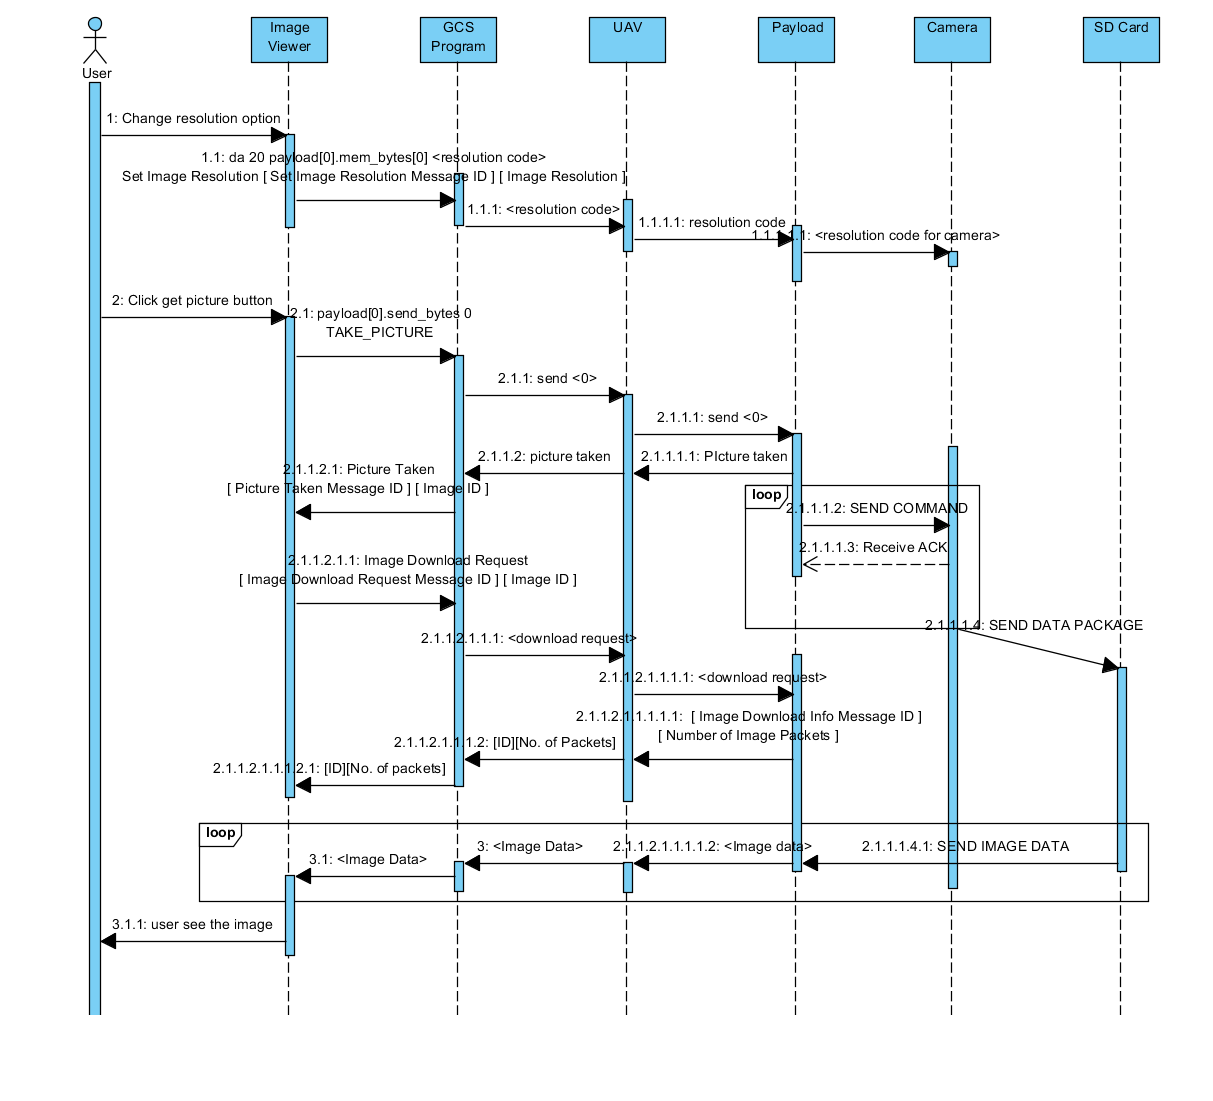
\includegraphics[width=1.00\textwidth]{figures/sequence_diagram.png} 
\end{center}
\caption{Sequence Diagram of the Data flow\label{sequence diagram}}
\end{figure}

Image data is also sent in the same basic manner, however the image is broken up into `packets' of data
which can be placed into the shared memory of the autopilot one at a time, as described by the \emph{Image Data}
message described above. One packet is sent for every transmit token sent by the autopilot, ensuring that the
payload module does not saturate the autopilot link with data. While packets are being sent, the main event loop
still checks for messages being sent from the ground station, allowing functionality such as the cancel download message 
to be implemented. In this way the payload module can transmit a whole image over the autopilot connection.

The testing of the image sending system is described in section \ref{sec:test_pl_image_send}, verifying the milestones 
as described.

Verification of milestone \ref{sec:ms_pl_img_gs_cam_res} (changing image resolution) can be seen in test \ref{sec:test_change_resolution}. Unfortunately changing colour type (milestone \ref{sec:ms_pl_img_gs_cam_colour_type})  was not fully implemented due to time constraints.

\subsection{Problems Encountered (mh)}
A number of problems were encountered and overcome during the implementation of the payload-ground station
communication code, a few of the most important are reproduced here.

\subsubsection*{Autopilot Bug (ab)}

The Autopilot sends "Transmit" tokens to the payload module every 20ms, 
to which a payload module sent an "ACK" token, even when it does not 
transmit any data. We encountered a problem whereby if our we tried to 
send any data to the payload during an "ACK", the autopilot would stop 
sending any "Transmit" tokens at all, effectively cutting off all 
communication to the payload module.

\begin{figure}[H]
  \centering
  \begin{tabular}{c c}
  \subfigure{\label{fig:testing_sc2_working1}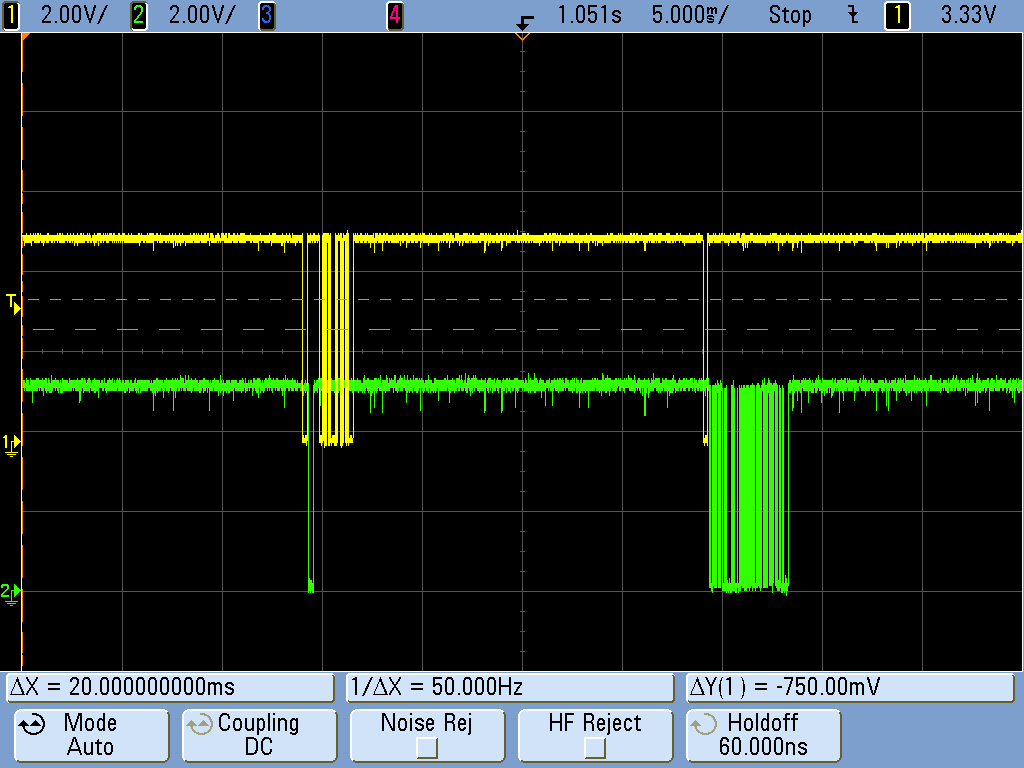
\includegraphics[width=0.5\textwidth]{scope/scope_1.png}}&                
  \subfigure{\label{fig:testing_sc2_working2}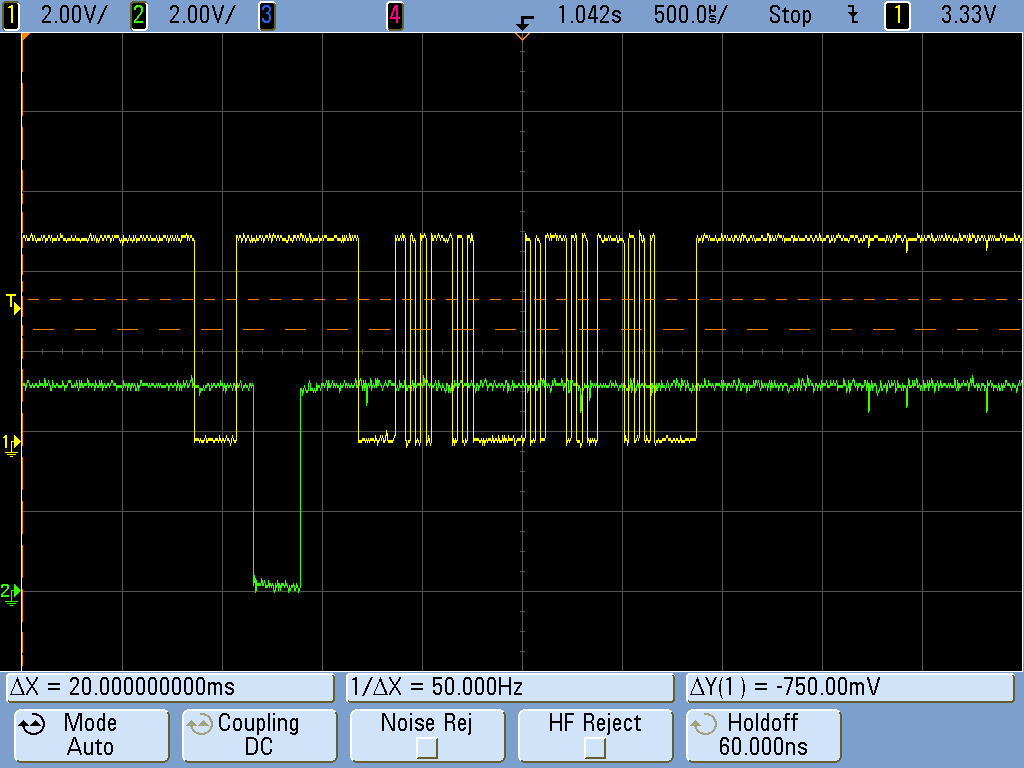
\includegraphics[width=0.5\textwidth]{scope/scope_2.png}} \\
  \subfigure{\label{fig:testing_sc2_working3}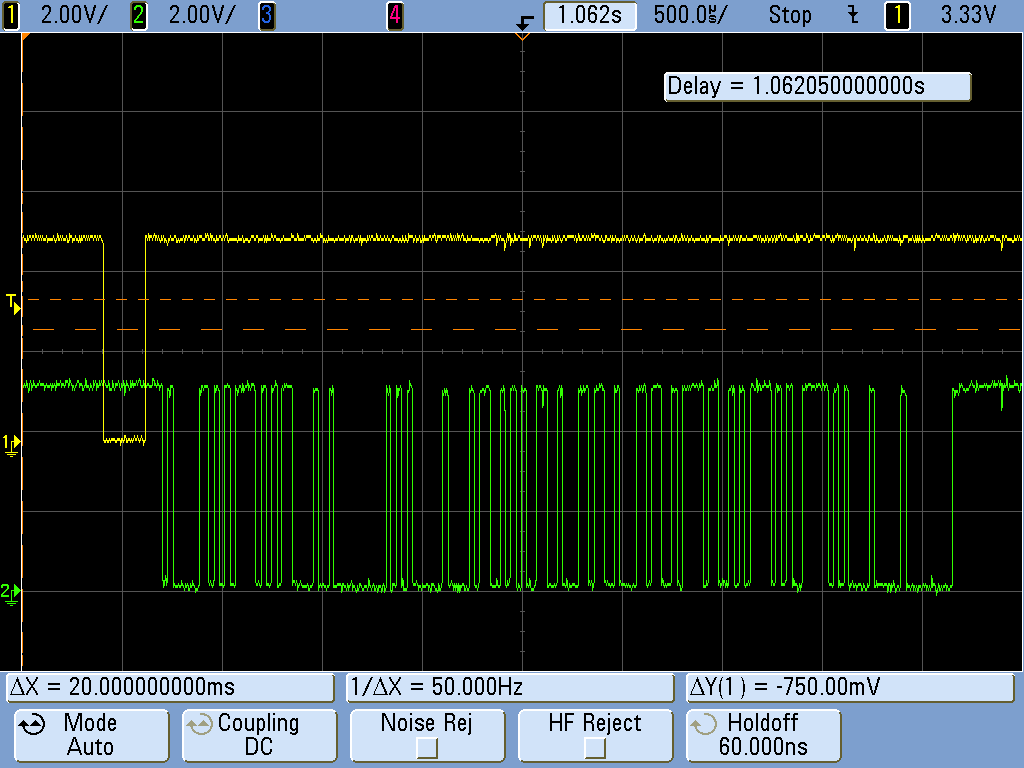
\includegraphics[width=0.5\textwidth]{scope/scope_3.png}}&                
  \subfigure{\label{fig:testing_sc2_working4}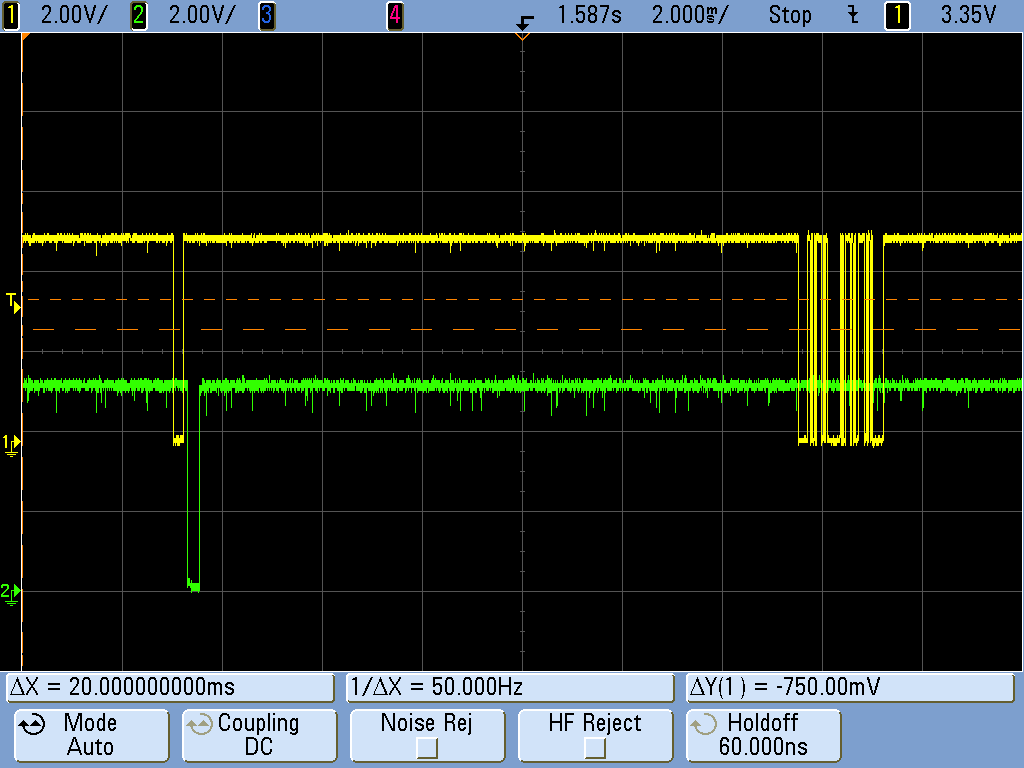
\includegraphics[width=0.5\textwidth]{scope/scope_11.png}}
  \end{tabular}
  \captionof{figure}{Oscilloscope traces for the situation where the autopilot does not break: In yellow is the Autopilot TX, in green the Payload TX. In this situation, after an ACK token is received by the autopilot, a SEND\_BYTES instruction is sent. On the next transmit token, a series of bytes is sent to the autopilot, and the autopilot continues to send Transmit tokens.}
  \label{fig:testing_sc2_working}
\end{figure}

\begin{figure}[H]
  \centering
  \begin{tabular}{c c}
  \subfigure{\label{fig:testing_sc2_broken1}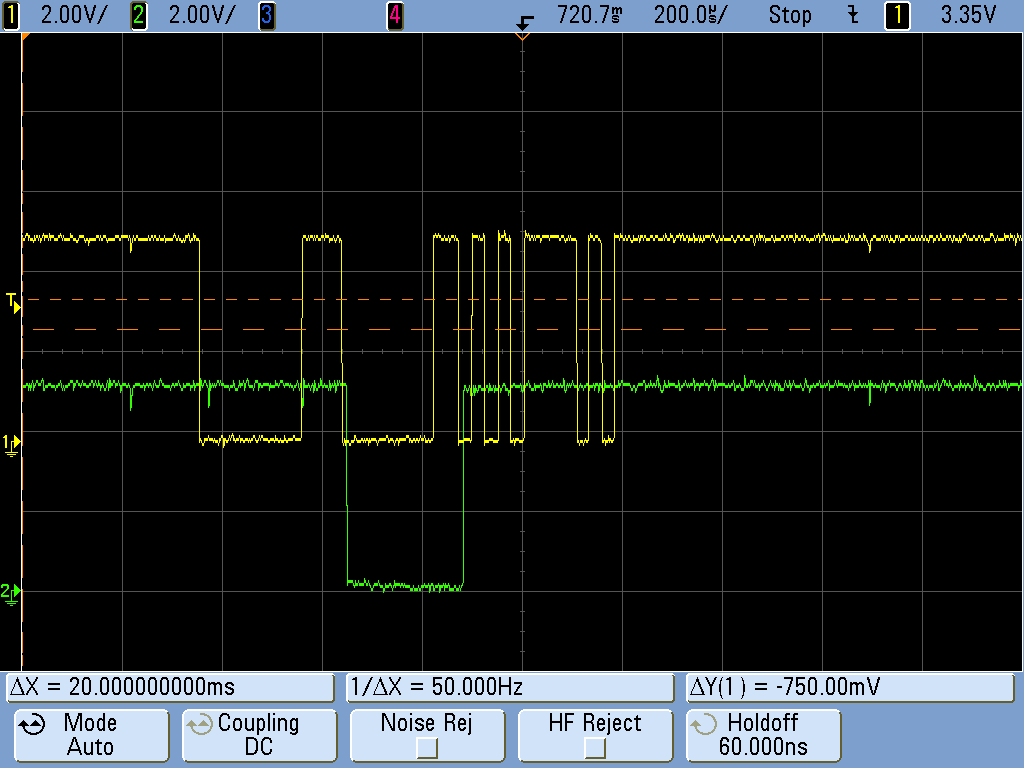
\includegraphics[width=0.5\textwidth]{scope/scope_6.png}}&                
  \subfigure{\label{fig:testing_sc2_broken2}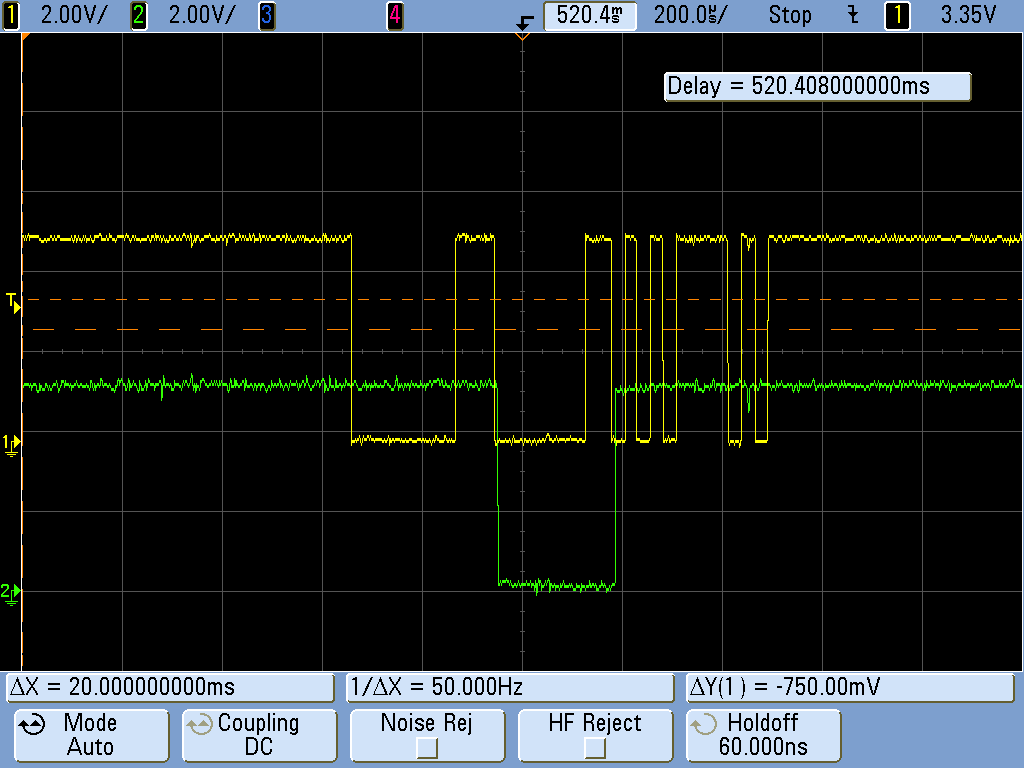
\includegraphics[width=0.5\textwidth]{scope/scope_14.png}} \\
  \subfigure{\label{fig:testing_sc2_broken3}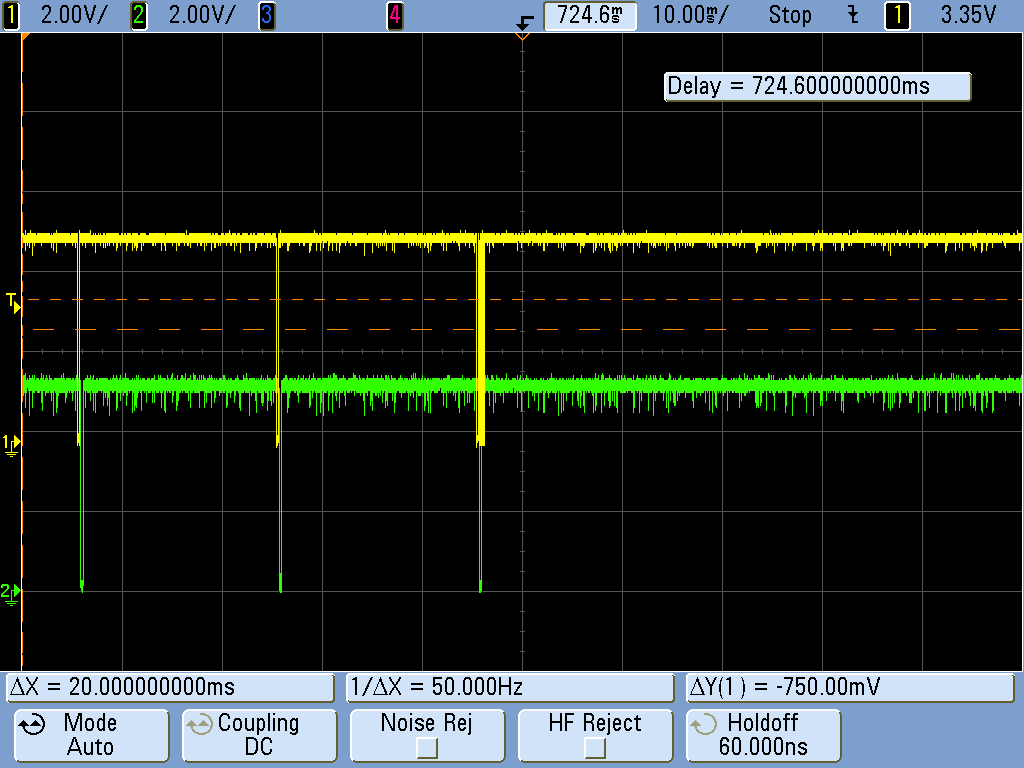
\includegraphics[width=0.5\textwidth]{scope/scope_7.png}}
  \end{tabular}
  \captionof{figure}{Oscilloscope traces for the situation where the autopilot breaks: In yellow is the Autopilot TX, in green the Payload TX. In this situation, whilst an ACK token is received by the autopilot, a SEND\_BYTES instruction is sent. No more transmit tokens are sent, therefore communication with the payload stops.}
  \label{fig:testing_sc2_broken}
\end{figure}

Not sure whether this was a bug with the Autopilot, we got in contact with 
our customer, sending all scope traces to him and a description of how 
to reproduce the error. Not being able to reproduce it with his dummy 
payload (strange, as our dummy payloads only differed in that his used a
surface-mount version of an ATmega168 and a MAX3070 transceiver instead 
of MAX489), he then came to ECS and debugged the Autopilot with us.

After a significant amount of time debugging the Autopilot and our 
payload, it was discovered this was indeed a problem with the Autopilot, 
which our customer was able to fix and subsequently update the firmware 
of our Autopilot.

\subsubsection*{Volatile Variables and ISRs (mh)}

Another problem encountered regarded a flag variable being checked in a function called in the main event loop. The flag
was the continuation condition of a while loop, and although it was being set in another section of code this new set 
value was not being propagated to the while loop code, meaning that the while loop would continue forever. This problem
was discovered (helped greatly by the debug interface described in section \ref{sec:payload_debug_interface}) . After some
consideration, research and experimentation it was discovered that the problem lay with the C compilers optimization. The 
flag was being set in a interrupt service routine (ISR), which the compiler assumed could not be called during the while loop
call, therefore it was optimized out, causing the loop to continue forever. The solution to this was to set this flag variable 
as \emph{volatile}, preventing it from being optimized out in this manner. The same was applied to all global variables modified in ISRs.


%|||||||| REMINDER: PROBLEMS CHALLENGES
%|||||||| REMINDER: HOW DID WE SOLVE PROBLEMS, DEBUGGING, TESTING, ETC
%|||||||| REMINDER: JOHN COULD TALK ABOUT HOW BROKEN CAMERAS SLOWED DOWN DEVELOPMENT BUT GOOD PLANNING AND CONTINGENCY MINIMISED RISK OR IN MANAGEMENT SECTION
%|||||||| REMINDER: FUTURE WORK
%|||||||| REMINDER: ADD NEWPAGES BETWEEN SECTIONS


